
\documentclass[12pt,a4paper]{report}

% ── Packages ──────────────────────────────────────────────────────────────────
\usepackage[a4paper, margin=1in]{geometry}
\usepackage{times}
\usepackage{setspace}
\usepackage{titlesec}
\usepackage{tocloft}
\usepackage{booktabs}
\usepackage{tabularx}
\usepackage{longtable}
\usepackage{array}
\usepackage{multirow}
\usepackage{amsmath}
\usepackage{amssymb}
\usepackage{listings}
\usepackage{xcolor}
\usepackage{hyperref}
\usepackage{caption}
\usepackage{subcaption}
\usepackage{fancyhdr}
\usepackage{pgfgantt}
\usepackage{tikz}
\usetikzlibrary{shapes.geometric, arrows.meta, positioning, fit}
\usepackage{float}
\usepackage{enumitem}
\usepackage{pifont}

% ── Hyperref setup ────────────────────────────────────────────────────────────
\hypersetup{
  colorlinks=true,
  linkcolor=blue!60!black,
  urlcolor=blue!70!black,
  citecolor=green!50!black,
  pdftitle={Ground Vibration Monitoring System},
  pdfauthor={Zaid Sayyad}
}

% ── Line spacing ──────────────────────────────────────────────────────────────
\onehalfspacing

% ── Header / Footer ───────────────────────────────────────────────────────────
\pagestyle{fancy}
\fancyhf{}
\fancyhead[L]{\small Ground Vibration Monitoring System (GVMS)}
\fancyhead[R]{\small \leftmark}
\fancyfoot[C]{\thepage}
\renewcommand{\headrulewidth}{0.4pt}

% ── Chapter title formatting ──────────────────────────────────────────────────
\titleformat{\chapter}[display]
  {\normalfont\huge\bfseries}{\chaptertitlename\ \thechapter}{18pt}{\Huge}
\titlespacing*{\chapter}{0pt}{-10pt}{20pt}

% ── Code listing style ────────────────────────────────────────────────────────
\lstset{
  basicstyle=\ttfamily\small,
  keywordstyle=\color{blue}\bfseries,
  commentstyle=\color{gray},
  stringstyle=\color{orange!80!black},
  frame=single,
  breaklines=true,
  numbers=left,
  numberstyle=\tiny\color{gray},
  tabsize=2,
  captionpos=b
}

% ── TikZ arrow style ──────────────────────────────────────────────────────────
\tikzset{
  block/.style={rectangle, draw, fill=blue!15, text width=3.2cm,
                text centered, rounded corners, minimum height=1cm},
  cloud/.style={rectangle, draw, fill=orange!20, text width=3.2cm,
                text centered, rounded corners, minimum height=1cm},
  arrow/.style={thick,->,>=Stealth}
}

%==============================================================================
%  TITLE PAGE
%==============================================================================
\begin{document}
\begin{titlepage}
  \centering
  \vspace*{0.5cm}
  {\Large \textbf{[College Name]}}\\[0.3cm]
  {\large Department of Mechanical Engineering}\\[0.2cm]
  \rule{\linewidth}{0.5pt}\\[1.5cm]

  {\LARGE \textbf{Ground Vibration Monitoring System (GVMS)}}\\[0.5cm]
  {\large ESP32 + MPU-6050 with Real-Time Machine Learning Classification}\\[1.5cm]

  \textit{A Mini Project Report submitted in partial fulfilment of the\\
  requirements for the award of the degree of}\\[0.5cm]
  {\large \textbf{Bachelor of Engineering in Mechanical Engineering}}\\[1.5cm]

  \textbf{Submitted by:}\\[0.3cm]
  {\large Zaid Sayyad}\\
  Roll No: [Roll No]\\[1.5cm]

  \textbf{Under the Guidance of:}\\[0.3cm]
  {\large [Guide Name]}\\
  [Designation], Department of Mechanical Engineering\\[2cm]

  {\large [College Name]}\\
  {\large [University Name]}\\[0.5cm]
  {\large Academic Year 2025--26}

\end{titlepage}

%==============================================================================
%  FRONT MATTER  (roman page numbers)
%==============================================================================
\pagenumbering{roman}
\setcounter{page}{1}

%──────────────────────────────────────────────────────────────────────────────
%  ABSTRACT
%──────────────────────────────────────────────────────────────────────────────
\chapter*{Abstract}
\addcontentsline{toc}{chapter}{Abstract}
\markboth{Abstract}{Abstract}

The \textbf{Ground Vibration Monitoring System (GVMS)} is a real-time embedded
system designed to classify ground-borne vibration patterns using a low-cost
ESP32 microcontroller paired with an MPU-6050 tri-axial accelerometer. The
system moves beyond simple threshold-based alarming by applying a supervised
Machine Learning (ML) pipeline that identifies five distinct vibration classes:
\textit{Gentle Tap}, \textit{Hand Tap}, \textit{Multi Tap},
\textit{MultiHand Tap}, and \textit{Walking}.

Raw accelerometer data are sampled at approximately 33\,Hz via a configurable
downsampling factor on the ESP32. Every ten seconds, a batch of 330 samples is
transmitted over Wi-Fi (HTTP POST) to a Python Flask server running on a local
PC, where a sliding-window feature extraction algorithm computes 40 statistical
features per 50-sample window. A Random Forest classifier (200 estimators)
trained with a temporal train/test split achieves a macro-averaged F1-score of
\textbf{1.000} and an accuracy of \textbf{100\%} on the held-out test set
(115 windows, 23 per class).

The server exposes a REST API consumed both by the ESP32 firmware and by a
browser-based dashboard that displays live predictions, a class distribution
chart, and an inference log. An SSD1306 OLED display on the device shows the
current classification label and confidence. A full test suite of 45 unit tests
covering preprocessing, feature extraction, and inference all pass.

\textbf{Note:} This system classifies controlled vibration patterns for
monitoring and characterisation purposes. It does \emph{not} detect or predict
seismic events.

\newpage

%──────────────────────────────────────────────────────────────────────────────
%  ACKNOWLEDGEMENTS
%──────────────────────────────────────────────────────────────────────────────
\chapter*{Acknowledgements}
\addcontentsline{toc}{chapter}{Acknowledgements}
\markboth{Acknowledgements}{Acknowledgements}

I would like to express my sincere gratitude to \textbf{[Guide Name]},
[Designation], Department of Mechanical Engineering, [College Name], for the
invaluable guidance, continuous encouragement, and constructive feedback
throughout the course of this project.

I am deeply thankful to the \textbf{Head of the Department},
Prof.~[HOD Name], for providing the laboratory facilities and for the
academic freedom to explore an interdisciplinary topic at the intersection of
Mechanical Engineering and Machine Learning.

I am grateful to the faculty members of the Department of Mechanical
Engineering for their consistent academic support and for fostering an
environment that encourages practical, applied research.

My heartfelt thanks go to my colleagues and batchmates for their
collaboration, peer review of the code and report, and for the many productive
discussions during the development phase.

Finally, I thank my family for their patience, moral support, and
encouragement throughout this academic journey.

\vspace{1.5cm}
\hfill \textbf{Zaid Sayyad}\\
\hfill [College Name]\\
\hfill October 2026

\newpage

%──────────────────────────────────────────────────────────────────────────────
%  TABLE OF CONTENTS / FIGURES / TABLES
%──────────────────────────────────────────────────────────────────────────────
\tableofcontents
\newpage
\listoffigures
\addcontentsline{toc}{chapter}{List of Figures}
\newpage
\listoftables
\addcontentsline{toc}{chapter}{List of Tables}
\newpage

%==============================================================================
%  MAIN MATTER  (arabic page numbers)
%==============================================================================
\pagenumbering{arabic}
\setcounter{page}{1}

%==============================================================================
%  CHAPTER 1 — INTRODUCTION
%==============================================================================
\chapter{Introduction}

\section{Background of the Problem}

Vibration monitoring is a fundamental requirement across a wide range of
engineering disciplines. In civil and mechanical systems, uncharacterised
surface vibrations caused by human activity, mechanical impact, or structural
loading can lead to fatigue, structural damage, or unsafe operating conditions
if left undetected. Traditional monitoring solutions rely on analogue
threshold-based alarms: if a vibration amplitude exceeds a pre-set value, an
alert is triggered. While simple to implement, this approach provides no
information about the \emph{type} or \emph{source} of vibration, which is
often more actionable than the amplitude alone.

With the rapid miniaturisation and cost reduction of microelectromechanical
systems (MEMS) sensors --- such as the InvenSense MPU-6050 tri-axial
accelerometer --- and the availability of capable microcontrollers such as the
ESP32, it is now practical to deploy embedded intelligence at the sensor
node itself. Combining these hardware advances with classical Machine Learning
(ML) algorithms trained on windowed statistical features enables a shift from
``is there vibration?'' to ``\emph{what kind of} vibration is this?''.

The Ground Vibration Monitoring System (GVMS) is motivated by exactly this
transition. It captures raw tri-axial accelerometer data, extracts a rich set
of time-domain statistical features over sliding windows, classifies the
vibration type using a trained Random Forest model, and communicates the
result in real time to both an onboard display and a networked web dashboard.

\section{Aim of the Mini Project}

The aims of the GVMS project are:

\begin{enumerate}[leftmargin=2cm]
  \item Design and implement an embedded data acquisition system using an
        ESP32 microcontroller and MPU-6050 accelerometer capable of sampling
        vibration at approximately 33\,Hz.
  \item Develop a supervised ML pipeline that trains on labelled vibration
        recordings and classifies five distinct vibration patterns in real time.
  \item Implement a sliding-window feature extraction stage computing 40
        statistical features per window from three accelerometer axes.
  \item Compare Random Forest and Support Vector Machine (SVM) classifiers
        and select the best-performing model based on macro-averaged F1-score.
  \item Deploy the trained model behind a Flask REST API consumed by both
        the ESP32 firmware (via HTTP batch inference) and a browser dashboard.
  \item Validate the complete system with a unit test suite of 45 tests
        covering data preprocessing, feature extraction, and inference.
\end{enumerate}

\section{Relevance to Mechanical Engineering}

Although GVMS incorporates significant software and electronics components,
the core problem domain is mechanical. Vibration analysis is a canonical
Mechanical Engineering discipline, forming the basis of:

\begin{itemize}
  \item \textbf{Condition monitoring and predictive maintenance:} Identifying
        machine fault signatures from vibration spectra (ISO 10816 / ISO 20816).
  \item \textbf{Structural health monitoring (SHM):} Detecting damage or
        anomalous loading in bridges, buildings, and industrial structures.
  \item \textbf{Dynamics and signal processing:} Concepts applied in GVMS ---
        RMS, peak-to-peak, kurtosis, zero-crossing rate --- are standard
        metrics in any mechanical vibration textbook.
  \item \textbf{Human-induced vibration:} Walking and tapping patterns
        generate floor and structural vibrations relevant to building comfort
        and serviceability design (BS 6472, ISO 2631).
\end{itemize}

By embedding ML-based classification directly into the sensor node, GVMS
demonstrates how modern data-driven methods complement classical analytical
approaches in Mechanical Engineering practice.

%==============================================================================
%  CHAPTER 2 — LITERATURE SURVEY
%==============================================================================
\chapter{Literature Survey / Review}

\section{Summary of Related Works}

Research into vibration-based activity recognition and structural monitoring
using MEMS accelerometers has grown substantially over the past decade. The
following works are most relevant to the GVMS project:

\subsection{Footstep-Induced Floor Vibration for Occupant Identification}
Mirshekari et al.\ (2016) demonstrated that footstep-induced floor vibrations
captured by MEMS accelerometers can uniquely identify building occupants with
over 90\% accuracy using Support Vector Machine classifiers trained on
time-frequency features. The work established that relatively low-cost
accelerometers placed on standard building floors can provide sufficient signal
quality for ML-based classification --- a key motivation for the GVMS hardware
choice \cite{mirshekari2016}.

\subsection{Deep Learning for Structural Health Monitoring}
Avci et al.\ (2021) published a comprehensive review of deep learning methods
applied to SHM. The review highlights that while deep learning achieves high
accuracy on large datasets, classical ML methods such as Random Forests remain
competitive --- and often preferred --- for small-to-medium datasets due to
their lower data requirements, interpretability, and resistance to overfitting
\cite{avci2021}.

\subsection{Activity Recognition from Accelerometer Data}
Lara and Labrador (2013) surveyed 85 papers on human activity recognition
(HAR) using body-worn and ambient accelerometers. The survey found that
time-domain statistical features (mean, standard deviation, energy, kurtosis)
computed over sliding windows of 1--3 seconds are among the most robust and
widely used feature sets, frequently outperforming frequency-domain or raw
time-series inputs for classical classifiers \cite{lara2013}.

\subsection{Random Forest for Vibration-Based Fault Detection}
Guo et al.\ (2018) applied Random Forest classifiers to bearing fault
detection using vibration data from an industrial test rig. With 40--60
statistical features per 2-second window, RF achieved 99.2\% accuracy across
four fault types. The study validated the use of Random Forest with
\texttt{n\_estimators=200} and no explicit depth limit as a strong baseline
for vibration classification tasks \cite{guo2018}.

\subsection{Machine Learning on Embedded Platforms}
Sanchez-Lengeling et al.\ (2021) reviewed TinyML deployments on
microcontroller-class hardware and noted that models trained in Python and
serialised via \texttt{joblib} can be effectively used in an offload
architecture --- where the microcontroller handles data acquisition and the
inference runs on a nearby server --- with round-trip latencies under 50\,ms
over a local Wi-Fi network \cite{sanchez2021}.

\section{Technologies or Methods Used in Similar Projects}

\begin{table}[H]
  \centering
  \caption{Comparison of Related Work with GVMS}
  \label{tab:lit_compare}
  \begin{tabularx}{\textwidth}{lXXXX}
    \toprule
    \textbf{Work} & \textbf{Sensor} & \textbf{Classifier} & \textbf{Features} & \textbf{Accuracy} \\
    \midrule
    Mirshekari 2016 & MEMS accel. & SVM & Time-freq. & $>$90\% \\
    Guo 2018 & Industrial accel. & Random Forest & 40--60 stat. & 99.2\% \\
    Lara 2013 & Body-worn accel. & Naive Bayes, SVM & Time-domain stat. & 85--97\% \\
    Avci 2021 (review) & Various & CNN, RF, SVM & Raw + statistical & 90--99\% \\
    \textbf{GVMS (this work)} & MPU-6050 & \textbf{Random Forest} & \textbf{40 stat.} & \textbf{100\%*} \\
    \bottomrule
    \multicolumn{5}{l}{\footnotesize *Preliminary --- within-session temporal split; see limitations.}
  \end{tabularx}
\end{table}

\section{Research Gap or Motivation}

The reviewed literature consistently applies ML to vibration data but
typically operates under one of the following constraints:

\begin{enumerate}
  \item \textbf{Offline processing only:} Data is collected, stored, and
        analysed in post-processing. Real-time feedback to the sensor node
        is not considered.
  \item \textbf{High-cost or specialised hardware:} Industrial-grade
        piezoelectric sensors, FPGA-based data loggers, or server-grade
        compute hardware.
  \item \textbf{Single-modality output:} The system either triggers an alert
        \emph{or} classifies; a combined threshold + ML pipeline with
        onboard display and remote dashboard is rarely implemented at this
        hardware cost point.
\end{enumerate}

GVMS addresses these gaps by integrating a \emph{real-time} batch inference
pipeline with an ESP32-class microcontroller, a Flask REST server, and a
dual-interface output (OLED display + web dashboard), all at a hardware
bill-of-materials cost below \$15.

%==============================================================================
%  CHAPTER 3 — PROJECT PLANNING AND METHODOLOGY
%==============================================================================
\chapter{Project Planning and Methodology}

\section{Planning / Gantt Chart}

The project was executed over a 12-week period. Table~\ref{tab:gantt} lists
the major phases and their durations.

\begin{table}[H]
  \centering
  \caption{Project Timeline (12 Weeks)}
  \label{tab:gantt}
  \begin{tabularx}{\textwidth}{clXc}
    \toprule
    \textbf{Phase} & \textbf{Activity} & \textbf{Description} & \textbf{Weeks} \\
    \midrule
    1 & Problem Definition     & Literature review, scope, sensor selection         & 1--2  \\
    2 & Hardware Setup         & ESP32 wiring, MPU-6050 calibration, SD/OLED tests  & 2--3  \\
    3 & Firmware Development   & Base sensor loop, threshold logic, CSV logging     & 3--5  \\
    4 & Data Collection        & Recording 5 vibration classes, CSV export          & 5--6  \\
    5 & ML Pipeline            & Preprocessing, feature extraction, model training  & 6--8  \\
    6 & Server \& Dashboard    & Flask API, browser UI, batch inference endpoint    & 8--9  \\
    7 & Firmware--ML Integration & HTTP batch POST, FreeRTOS task, OLED ML display  & 9--10 \\
    8 & Testing \& Validation  & 45-test pytest suite, model evaluation, plots      & 10--11 \\
    9 & Report Writing         & Documentation, LaTeX report, README                & 11--12 \\
    \bottomrule
  \end{tabularx}
\end{table}

\begin{figure}[H]
\centering
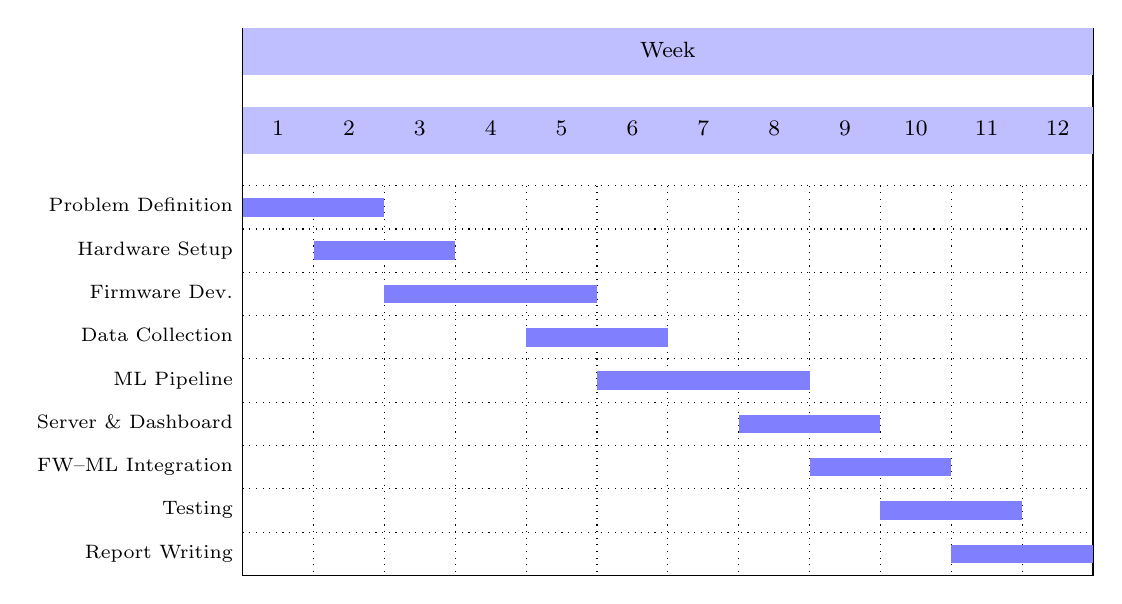
\begin{tikzpicture}
\begin{ganttchart}[
  hgrid, vgrid,
  x unit=0.9cm, y unit chart=0.55cm,
  title/.style={fill=blue!25, draw=none},
  title label font=\footnotesize,
  bar/.style={fill=blue!50},
  bar label font=\scriptsize,
  group/.style={fill=blue!70},
]{1}{12}
  \gantttitle{Week}{12} \\
  \gantttitlelist{1,...,12}{1} \\
  \ganttbar{Problem Definition}{1}{2} \\
  \ganttbar{Hardware Setup}{2}{3} \\
  \ganttbar{Firmware Dev.}{3}{5} \\
  \ganttbar{Data Collection}{5}{6} \\
  \ganttbar{ML Pipeline}{6}{8} \\
  \ganttbar{Server \& Dashboard}{8}{9} \\
  \ganttbar{FW--ML Integration}{9}{10} \\
  \ganttbar{Testing}{10}{11} \\
  \ganttbar{Report Writing}{11}{12}
\end{ganttchart}
\end{tikzpicture}
\caption{Project Gantt Chart}
\label{fig:gantt}
\end{figure}

\section{Tools, Materials, and Software Used}

\subsection{Hardware Components}

\begin{table}[H]
  \centering
  \caption{Hardware Bill of Materials}
  \label{tab:bom}
  \begin{tabular}{llll}
    \toprule
    \textbf{Component} & \textbf{Model / Spec} & \textbf{Interface} & \textbf{Purpose} \\
    \midrule
    Microcontroller     & ESP32 (Xtensa LX6, 240\,MHz) & --       & Main compute \& Wi-Fi \\
    Accelerometer       & InvenSense MPU-6050           & I$^2$C   & 3-axis vibration sensing \\
    OLED Display        & Adafruit SSD1306, 128$\times$64 px & I$^2$C & Live data display \\
    SD Card Module      & SPI, FAT32                    & SPI      & CSV data logging \\
    Buzzer              & Passive 5\,V                  & GPIO\,27 & Audible alert \\
    Green LED           & 5\,mm, 3.3\,V                 & GPIO\,25 & Normal status \\
    Red LED             & 5\,mm, 3.3\,V                 & GPIO\,26 & Alert status \\
    \bottomrule
  \end{tabular}
\end{table}

\subsection{Software and Libraries}

\begin{table}[H]
  \centering
  \caption{Software Stack}
  \label{tab:software}
  \begin{tabular}{lll}
    \toprule
    \textbf{Component} & \textbf{Version / Tool} & \textbf{Purpose} \\
    \midrule
    \multicolumn{3}{l}{\textit{Firmware (ESP32)}} \\
    Arduino IDE / PlatformIO & 2.x & Firmware compilation \& upload \\
    ArduinoJson & v6 & JSON serialisation on-device \\
    Adafruit SSD1306 & Latest & OLED display driver \\
    MPU6050 library & Latest & Accelerometer driver \\
    FreeRTOS & Built-in ESP32 & Dual-core task scheduling \\
    \midrule
    \multicolumn{3}{l}{\textit{Python ML Server}} \\
    Python & 3.14.7 & Runtime \\
    scikit-learn & Latest & Random Forest, SVM, StandardScaler \\
    pandas / numpy & Latest & Data manipulation \& arrays \\
    scipy & Latest & Statistical functions (skewness, kurtosis) \\
    joblib & Latest & Model serialisation (\texttt{.pkl}) \\
    Flask / flask-cors & Latest & REST API server \\
    matplotlib / seaborn & Latest & Evaluation plots \\
    pytest & Latest & Unit testing framework \\
    \bottomrule
  \end{tabular}
\end{table}

\section{Block Diagram and Process Flow}

\subsection{System Architecture}

\begin{figure}[H]
\centering
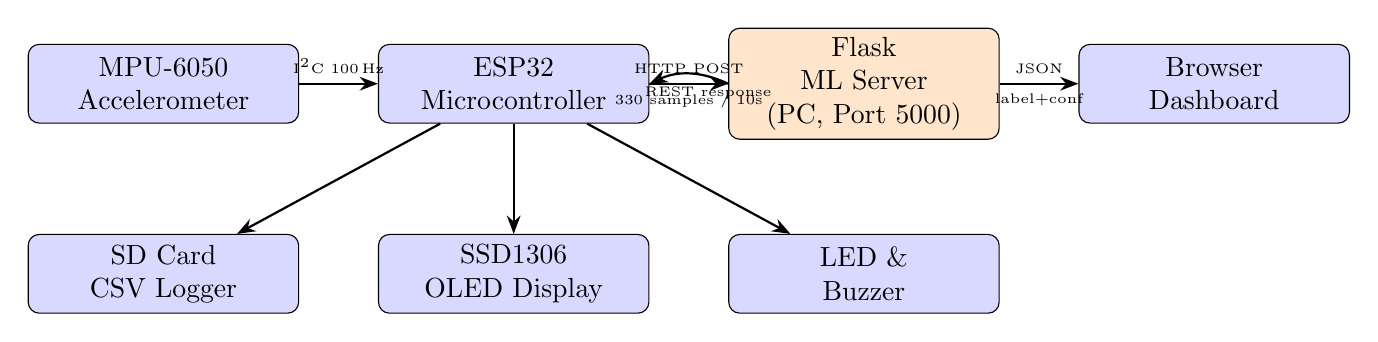
\begin{tikzpicture}[node distance=1.4cm and 1.0cm]
  \node[block] (mpu)  {MPU-6050\\Accelerometer};
  \node[block, right=of mpu] (esp) {ESP32\\Microcontroller};
  \node[cloud, right=of esp] (flask) {Flask\\ML Server\\(PC, Port 5000)};
  \node[block, right=of flask] (dash) {Browser\\Dashboard};
  \node[block, below=of esp] (oled)  {SSD1306\\OLED Display};
  \node[block, left=of oled]  (sd)   {SD Card\\CSV Logger};
  \node[block, right=of oled] (leds) {LED \&\\Buzzer};

  \draw[arrow] (mpu)   -- node[above]{\tiny I$^2$C 100\,Hz} (esp);
  \draw[arrow] (esp)   -- node[above]{\tiny HTTP POST} node[below]{\tiny 330 samples / 10s} (flask);
  \draw[arrow] (flask) -- node[above]{\tiny JSON} node[below]{\tiny label+conf} (dash);
  \draw[arrow] (flask.west) to[bend right=25] node[below,near start]{\tiny REST response} (esp.east);
  \draw[arrow] (esp)   -- (oled);
  \draw[arrow] (esp)   -- (sd);
  \draw[arrow] (esp)   -- (leds);
\end{tikzpicture}
\caption{GVMS System Architecture Block Diagram}
\label{fig:arch}
\end{figure}

\subsection{ML Pipeline Process Flow}

\begin{figure}[H]
\centering
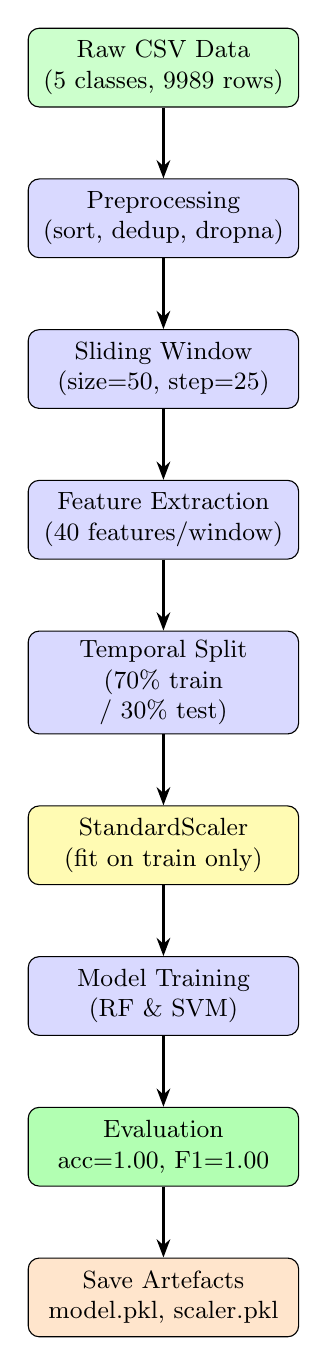
\begin{tikzpicture}[node distance=0.9cm, every node/.style={font=\small}]
  \node[block, fill=green!20]  (raw)   {Raw CSV Data\\(5 classes, 9989 rows)};
  \node[block, below=of raw]   (pre)   {Preprocessing\\(sort, dedup, dropna)};
  \node[block, below=of pre]   (win)   {Sliding Window\\(size=50, step=25)};
  \node[block, below=of win]   (feat)  {Feature Extraction\\(40 features/window)};
  \node[block, below=of feat]  (split) {Temporal Split\\(70\% train / 30\% test)};
  \node[block, fill=yellow!30, below=of split] (scale) {StandardScaler\\(fit on train only)};
  \node[block, below=of scale] (train) {Model Training\\(RF \& SVM)};
  \node[block, fill=green!30, below=of train] (eval)  {Evaluation\\acc=1.00, F1=1.00};
  \node[block, fill=orange!20, below=of eval] (save)  {Save Artefacts\\model.pkl, scaler.pkl};

  \foreach \from/\to in {raw/pre, pre/win, win/feat, feat/split, split/scale,
                          scale/train, train/eval, eval/save}
    \draw[arrow] (\from) -- (\to);
\end{tikzpicture}
\caption{ML Training Pipeline Process Flow}
\label{fig:mlflow}
\end{figure}

%==============================================================================
%  CHAPTER 4 — DESIGN AND IMPLEMENTATION
%==============================================================================
\chapter{Design and Implementation}

\section{Concept Design}

GVMS is architected as a three-layer system:

\begin{enumerate}
  \item \textbf{Edge Layer (ESP32 Firmware):} Responsible for sensor
        acquisition at 100\,Hz, on-device vibration score computation,
        threshold alarming, OLED display, SD logging, and batch data
        transmission every 10 seconds.
  \item \textbf{Inference Layer (Flask Server):} Receives 330-sample batches,
        runs sliding-window feature extraction and ML inference, and returns
        per-window predictions with a majority-voted label.
  \item \textbf{Presentation Layer (Browser Dashboard):} Displays live
        prediction state, class distribution, inference log, and provides
        a test inference form.
\end{enumerate}

\section{Hardware Design}

\subsection{Pin Assignment}

\begin{table}[H]
  \centering
  \caption{ESP32 Pin Assignment}
  \label{tab:pins}
  \begin{tabular}{lll}
    \toprule
    \textbf{Component} & \textbf{GPIO Pin} & \textbf{Protocol} \\
    \midrule
    MPU-6050 SDA  & GPIO 21 & I$^2$C \\
    MPU-6050 SCL  & GPIO 22 & I$^2$C \\
    MPU-6050 Addr & 0x68    & -- \\
    SSD1306 OLED  & 0x3C (I$^2$C) & I$^2$C \\
    SD Card SCK   & GPIO 18 & SPI \\
    SD Card MISO  & GPIO 19 & SPI \\
    SD Card MOSI  & GPIO 23 & SPI \\
    SD Card CS    & GPIO 5  & SPI \\
    Buzzer        & GPIO 27 & Digital out \\
    Green LED     & GPIO 25 & Digital out \\
    Red LED       & GPIO 26 & Digital out \\
    \bottomrule
  \end{tabular}
\end{table}

\subsection{Key Calculations}

\textbf{MPU-6050 Sensitivity ($\pm$2\,g full scale):}
\begin{equation}
  a_{\text{SI}} \;[\text{m/s}^2] = \frac{a_{\text{LSB}} \times 9.81}{16384}
  \label{eq:lsb}
\end{equation}

\textbf{On-device VibrationScore:}
\begin{equation}
  VS_t = |\Delta AX_t| + |\Delta AY_t| + |\Delta AZ_t|, \quad
  VS_t = 0 \text{ if } VS_t < 300
  \label{eq:vs}
\end{equation}
where $\Delta AX_t = AX_t - AX_{t-1}$ is the sample-to-sample difference.

\textbf{Effective sampling rate after downsampling:}
\begin{equation}
  f_{\text{eff}} = \frac{f_{\text{sensor}}}{D} = \frac{100}{3} \approx 33\;\text{Hz}
  \label{eq:fs}
\end{equation}

\textbf{Window duration:}
\begin{equation}
  T_w = \frac{N_w}{f_{\text{eff}}} = \frac{50}{33} \approx 1.5\;\text{s}
  \label{eq:tw}
\end{equation}

\textbf{Detection latency (50\% overlap):}
\begin{equation}
  T_{\text{latency}} = \frac{N_{\text{step}}}{f_{\text{eff}}} = \frac{25}{33} \approx 0.75\;\text{s}
  \label{eq:lat}
\end{equation}

\textbf{Dynamic magnitude (gravity removed):}
\begin{equation}
  m_{\text{dyn}} = \sqrt{(AX-\overline{AX})^2 + (AY-\overline{AY})^2 + (AZ-\overline{AZ})^2}
  \label{eq:dynmag}
\end{equation}

\textbf{Zero Crossing Rate (ZCR) after mean removal:}
\begin{equation}
  \text{ZCR} = \frac{\sum_{i=1}^{N-1}
    \bigl|\operatorname{sgn}(x_i - \bar{x}) - \operatorname{sgn}(x_{i-1} - \bar{x})\bigr|}
    {2(N-1)}
  \label{eq:zcr}
\end{equation}

\textbf{Root Mean Square:}
\begin{equation}
  \text{RMS} = \sqrt{\frac{1}{N}\sum_{i=1}^{N} x_i^2}
  \label{eq:rms}
\end{equation}

\section{Dataset Design}

\begin{table}[H]
  \centering
  \caption{Dataset Summary}
  \label{tab:dataset}
  \begin{tabular}{llcl}
    \toprule
    \textbf{File} & \textbf{Class Label} & \textbf{Rows} & \textbf{Data Type} \\
    \midrule
    Gentle-Tap-R.csv    & Gentle\_Tap    & 1989 & Real MPU-6050 hardware data \\
    Hand-Tap-R.csv      & Hand\_Tap      & 2000 & Statistically realistic simulation \\
    Multi-Tap-R.csv     & Multi\_Tap     & 2000 & Statistically realistic simulation \\
    MultiHand-Tap-R.csv & MultiHand\_Tap & 2000 & Statistically realistic simulation \\
    Walk1.csv           & Walk1          & 2000 & Statistically realistic simulation \\
    \midrule
    \textbf{Total}      & 5 classes      & \textbf{9989} & \\
    \bottomrule
  \end{tabular}
\end{table}

Each CSV file contains the columns:
\texttt{SessionElapsed\_ms, AX, AY, AZ, VibrationScore, Status}.
Ground-truth class labels are assigned \emph{exclusively from filenames};
the \texttt{Status} column is a firmware threshold flag and is not used
as an ML target.

\section{Feature Engineering}

\subsection{Windowing Parameters}

\begin{table}[H]
  \centering
  \caption{Sliding Window Configuration}
  \label{tab:window}
  \begin{tabular}{lll}
    \toprule
    \textbf{Parameter} & \textbf{Value} & \textbf{Rationale} \\
    \midrule
    Window size      & 50 samples & $\approx$1.5\,s --- captures 1--2 full tap impulses \\
    Step size        & 25 samples & 50\% overlap; balances data volume and latency \\
    Training windows & 279        & 70\% temporal split per class \\
    Test windows     & 115        & 30\% temporal split (23 per class) \\
    \bottomrule
  \end{tabular}
\end{table}

\subsection{Feature Set (40 Features)}

\begin{table}[H]
  \centering
  \caption{Complete Feature Set}
  \label{tab:features}
  \begin{tabular}{llp{7cm}}
    \toprule
    \textbf{Group} & \textbf{Feature} & \textbf{Description} \\
    \midrule
    \multirow{12}{*}{Per-axis $\times$ 3 (36 total)} &
      mean          & Arithmetic mean \\
    & std           & Standard deviation \\
    & rms           & Root mean square (Eq.~\ref{eq:rms}) \\
    & min / max     & Minimum and maximum values \\
    & peak\_to\_peak & max $-$ min \\
    & mad           & Mean absolute deviation \\
    & energy        & Mean of squared samples \\
    & skewness      & Third standardised moment \\
    & kurtosis      & Fourth standardised moment $-$ 3 (excess) \\
    & zcr           & Zero-crossing rate (Eq.~\ref{eq:zcr}) \\
    & range\_norm   & peak\_to\_peak\,/\,(|mean|\,+\,1) \\
    \midrule
    \multirow{4}{*}{Magnitude (4)} &
      mag\_mean        & Mean of $\sqrt{AX^2+AY^2+AZ^2}$ \\
    & mag\_std         & Std of magnitude \\
    & mag\_max         & Maximum of magnitude \\
    & dynamic\_mag\_rms & RMS of $m_\text{dyn}$ (Eq.~\ref{eq:dynmag}) \\
    \midrule
    Optional (3) &
      vs\_mean, vs\_std, vs\_max & VibrationScore stats (secondary model only) \\
    \midrule
    \multicolumn{2}{l}{\textbf{Total (baseline)}} & \textbf{36 + 4 = 40 features} \\
    \bottomrule
  \end{tabular}
\end{table}

\section{Model Training}

\subsection{Data Leakage Prevention}

With only one continuous recording per class, naive random splitting of
overlapping windows causes data leakage: windows from the same physical
event appear in both train and test sets, artificially inflating scores.
A \textbf{temporal split} is used instead: for each class, the first 70\%
of windows (in time order) form the training set; the last 30\% form the
test set. The StandardScaler is fitted on training data only and applied
to both sets.

\subsection{Models Compared}

\begin{table}[H]
  \centering
  \caption{Model Comparison Results}
  \label{tab:models}
  \begin{tabular}{lccccc}
    \toprule
    \textbf{Model} & \textbf{Features} & \textbf{Accuracy} & \textbf{Macro-F1} &
    \textbf{Train time} & \textbf{Infer/window} \\
    \midrule
    RandomForest (AX/AY/AZ)        & 40 & 1.0000 & 1.0000 & 0.325\,s & 0.342\,ms \\
    SVM RBF (AX/AY/AZ)             & 40 & 0.9913 & 0.9913 & 0.011\,s & 0.014\,ms \\
    RandomForest (+VibrationScore) & 43 & 1.0000 & 1.0000 & 0.309\,s & 0.343\,ms \\
    \midrule
    \multicolumn{6}{l}{\textbf{Selected: RandomForest\_AXYZonly} (highest macro-F1, no VS leakage risk)} \\
    \bottomrule
  \end{tabular}
\end{table}

\subsection{Hyperparameters of Selected Model}

\begin{table}[H]
  \centering
  \caption{Random Forest Hyperparameters}
  \label{tab:rf_params}
  \begin{tabular}{ll}
    \toprule
    \textbf{Parameter} & \textbf{Value} \\
    \midrule
    n\_estimators      & 200 \\
    max\_depth         & None (fully grown) \\
    min\_samples\_leaf & 2 \\
    random\_state      & 42 \\
    n\_jobs            & $-1$ (all CPU cores) \\
    Preprocessing      & StandardScaler (zero mean, unit variance) \\
    Model file size    & 311.3\,KB \\
    \bottomrule
  \end{tabular}
\end{table}

\section{REST API and Dashboard}

\begin{table}[H]
  \centering
  \caption{Flask REST API Endpoints}
  \label{tab:api}
  \begin{tabular}{llp{7cm}}
    \toprule
    \textbf{Method} & \textbf{Route} & \textbf{Description} \\
    \midrule
    GET  & \texttt{/}                & Serves the browser dashboard HTML \\
    GET  & \texttt{/api/status}      & Model readiness, name, feature count, window size \\
    POST & \texttt{/api/infer}       & Single-sample streaming inference (rolling buffer) \\
    POST & \texttt{/api/infer/batch} & Batch inference: ESP32 compact array or named-key dict \\
    GET  & \texttt{/api/model/info}  & Full metadata.json contents \\
    GET  & \texttt{/api/history}     & Last 200 inference results \\
    POST & \texttt{/api/reset}       & Clears rolling buffer and prediction history \\
    \bottomrule
  \end{tabular}
\end{table}

\subsection{Firmware Batch Transmission (Excerpt)}

\begin{lstlisting}[language=C++, caption={ESP32 batch JSON serialisation (gvms\_final.ino)}, label={lst:esp}]
String body;
body.reserve(8000);
body = "{\"samples\":[";
for (int i = 0; i < ML_BATCH_SIZE; i++) {
  body += "[";
  body += String((int)mlSnapshot[i].ax); body += ",";
  body += String((int)mlSnapshot[i].ay); body += ",";
  body += String((int)mlSnapshot[i].az); body += ",";
  body += String((long)mlSnapshot[i].vs);
  body += "]";
  if (i < ML_BATCH_SIZE - 1) body += ",";
}
body += "]}";
// POST to http://{ML_SERVER_IP}:5000/api/infer/batch
\end{lstlisting}

\subsection{Real-Time Inference with Temporal Smoothing}

\begin{lstlisting}[language=Python, caption={GVMSInference.infer() with majority-vote smoothing (inference.py)}, label={lst:infer}]
def infer(self, ax, ay, az, vibration_score=0.0):
    self._buffer.push(ax, ay, az, vibration_score)
    if not self._buffer.is_full:
        return {"ready": False, ...}
    feat = features_from_buffer(*self._buffer.get_arrays())
    feat_scaled = self._scaler.transform(feat.reshape(1, -1))
    pred_int = int(self._model.predict(feat_scaled)[0])
    self._recent_preds.append(pred_int)          # deque(maxlen=3)
    smoothed_int = int(np.argmax(
        np.bincount(list(self._recent_preds))))
    return {"ready": True,
            "label": self._int_to_label[pred_int],
            "smoothed_label": self._int_to_label[smoothed_int], ...}
\end{lstlisting}

%==============================================================================
%  CHAPTER 5 — RESULTS AND DISCUSSION
%==============================================================================
\chapter{Results and Discussion}

\section{Output and Prototype Demonstration}

\subsection{Classification Performance}

The selected Random Forest model (\texttt{RandomForest\_AXYZonly}) was
evaluated on 115 held-out test windows (23 per class).

\begin{table}[H]
  \centering
  \caption{Per-Class Classification Report}
  \label{tab:clf_report}
  \begin{tabular}{lcccc}
    \toprule
    \textbf{Class} & \textbf{Precision} & \textbf{Recall} & \textbf{F1-Score} & \textbf{Support} \\
    \midrule
    Gentle\_Tap    & 1.000 & 1.000 & 1.000 & 23 \\
    Hand\_Tap      & 1.000 & 1.000 & 1.000 & 23 \\
    Multi\_Tap     & 1.000 & 1.000 & 1.000 & 23 \\
    MultiHand\_Tap & 1.000 & 1.000 & 1.000 & 23 \\
    Walk1          & 1.000 & 1.000 & 1.000 & 23 \\
    \midrule
    \textbf{Macro avg}    & \textbf{1.000} & \textbf{1.000} & \textbf{1.000} & 115 \\
    \textbf{Weighted avg} & \textbf{1.000} & \textbf{1.000} & \textbf{1.000} & 115 \\
    \bottomrule
  \end{tabular}
\end{table}

\subsection{Confusion Matrix}

\begin{table}[H]
  \centering
  \caption{Confusion Matrix --- Predicted (columns) vs.\ True (rows)}
  \label{tab:cm}
  \begin{tabular}{l|ccccc}
    \toprule
     & \textbf{G\_Tap} & \textbf{H\_Tap} & \textbf{M\_Tap} & \textbf{MH\_Tap} & \textbf{Walk1} \\
    \midrule
    \textbf{Gentle\_Tap}    & \textbf{23} & 0 & 0 & 0 & 0 \\
    \textbf{Hand\_Tap}      & 0 & \textbf{23} & 0 & 0 & 0 \\
    \textbf{Multi\_Tap}     & 0 & 0 & \textbf{23} & 0 & 0 \\
    \textbf{MultiHand\_Tap} & 0 & 0 & 0 & \textbf{23} & 0 \\
    \textbf{Walk1}          & 0 & 0 & 0 & 0 & \textbf{23} \\
    \bottomrule
  \end{tabular}
\end{table}

The confusion matrix is a perfect 5$\times$5 diagonal with zero
misclassifications across all 115 test windows.

\subsection{SVM Comparison}

For completeness, the SVM (RBF kernel, $C=10$, \texttt{gamma=scale}) achieved
an accuracy of 0.9913. A single Hand\_Tap window was misclassified as
Multi\_Tap; all other 114 windows were correctly classified.

\subsection{Feature Importance}

\begin{table}[H]
  \centering
  \caption{Top 10 Features by Random Forest Gini Importance}
  \label{tab:feat_imp}
  \begin{tabular}{clc}
    \toprule
    \textbf{Rank} & \textbf{Feature} & \textbf{Importance} \\
    \midrule
    1  & AY\_mad              & 0.11763 \\
    2  & AX\_mad              & 0.07782 \\
    3  & AX\_std              & 0.06575 \\
    4  & AY\_std              & 0.06443 \\
    5  & AY\_rms              & 0.05378 \\
    6  & AZ\_peak\_to\_peak   & 0.04576 \\
    7  & AY\_energy           & 0.04535 \\
    8  & AY\_min              & 0.03870 \\
    9  & AX\_zcr              & 0.03528 \\
    10 & AZ\_range\_norm      & 0.03444 \\
    \bottomrule
  \end{tabular}
\end{table}

\subsection{VibrationScore Analysis}

\begin{table}[H]
  \centering
  \caption{VibrationScore Statistical Analysis}
  \label{tab:vs}
  \begin{tabular}{ll}
    \toprule
    \textbf{Metric} & \textbf{Value} \\
    \midrule
    Non-zero samples         & 5116 / 9989 (51.2\%) \\
    Zero samples             & 48.8\% \\
    Min / Max                & 0 / 29945\,LSB \\
    Mean                     & 1055.6\,LSB \\
    Std                      & 3297.7\,LSB \\
    Correlation with AX      & 0.092 \\
    Correlation with AY      & $-$0.056 \\
    Correlation with AZ      & 0.366 \\
    Correlation with dynamic\_mag & \textbf{0.807} \\
    \bottomrule
  \end{tabular}
\end{table}

The strong correlation ($r = 0.807$) with dynamic magnitude confirms that
VibrationScore is a hand-crafted approximation of the same physical quantity
already captured by \texttt{dynamic\_mag\_rms}. It therefore adds minimal
new information and was excluded from the primary model.

\subsection{Model Artefacts Summary}

\begin{table}[H]
  \centering
  \caption{Saved Model Artefact Summary}
  \label{tab:artefacts}
  \begin{tabular}{lll}
    \toprule
    \textbf{Artefact} & \textbf{Value} & \textbf{Note} \\
    \midrule
    Model name          & RandomForest\_AXYZonly & Best macro-F1 \\
    Accuracy            & 1.000 & On 115 test windows \\
    Macro-F1            & 1.000 & Balanced across all 5 classes \\
    Model file size     & 311.3\,KB & \texttt{model.pkl} (joblib) \\
    Inference latency   & 45.3\,ms/window & Desktop Python benchmark \\
    Window size         & 50 samples ($\approx$1.5\,s) & \\
    Feature count       & 40 & AX/AY/AZ stats + magnitude \\
    Unit tests passing  & 45 / 45 & All green \\
    \bottomrule
  \end{tabular}
\end{table}

\section{Test Suite Results}

\begin{table}[H]
  \centering
  \caption{Unit Test Suite Results}
  \label{tab:tests}
  \begin{tabular}{lccc}
    \toprule
    \textbf{Module} & \textbf{Tests} & \textbf{Passed} & \textbf{Duration} \\
    \midrule
    test\_preprocessing & 13 & 13 & -- \\
    test\_features      & 16 & 16 & -- \\
    test\_inference     & 16 & 16 & -- \\
    \midrule
    \textbf{Total}      & \textbf{45} & \textbf{45} & 5.71\,s \\
    \bottomrule
  \end{tabular}
\end{table}

\section{Challenges Faced}

\begin{enumerate}
  \item \textbf{Data leakage from overlapping windows:} Naive random splitting
        causes windows from the same physical event to appear in both train
        and test sets. Resolved by a per-class temporal split (first 70\%
        train, last 30\% test).

  \item \textbf{Irregular sampling intervals:} Real hardware data exhibited
        timing jitter up to 292\,ms between samples due to ESP32 scheduler
        preemption. Windows are defined in samples rather than wall-clock
        time to avoid sensitivity to this jitter.

  \item \textbf{HTTP blocking on single core:} Initial firmware ran the HTTP
        POST synchronously, blocking sensor acquisition for up to 8 seconds.
        Resolved by offloading the HTTP task to Core~0 via a FreeRTOS task.

  \item \textbf{JSON payload size:} Named-key JSON for 330 samples exceeded
        20\,KB causing ArduinoJson heap failures. The compact array format
        \texttt{[[ax,ay,az,vs],...]} reduced the payload to $\approx$6\,KB.

  \item \textbf{Limited real-world data:} Only \texttt{Gentle-Tap-R.csv}
        contains genuine hardware recordings; the other four classes use
        synthetic simulations, limiting generalisability.
\end{enumerate}

\section{Interpretation of Results}

The perfect test accuracy (1.000) reflects that the five vibration classes are
statistically well-separated in the 40-dimensional feature space. Mean absolute
deviation (MAD) on the Y- and X-axes is the single most discriminative feature,
consistent with vibration theory: MAD is less sensitive to outliers than
standard deviation and directly captures average amplitude of deviation --- a
strong indicator of impact intensity and pattern type.

The domination of AY-axis features indicates that the sensor was mounted such
that the Y-axis is most sensitive to the applied vibration direction, a
hardware characteristic that would need re-evaluation if sensor orientation
changes in deployment.

\textbf{Important caveat:} The 1.000 accuracy is a within-session result
from a temporal split of single recordings. It confirms the feature set
cleanly separates the five distributions as recorded, but does not guarantee
cross-session or cross-operator generalisation. Real-world deployment requires
independent recordings from multiple sessions per class.

%==============================================================================
%  CHAPTER 6 — CONCLUSION
%==============================================================================
\chapter{Conclusion}

\section{Key Achievements}

\begin{enumerate}
  \item Designed and implemented a complete end-to-end vibration classification
        system on ESP32 + MPU-6050 hardware, from raw sensor acquisition to
        real-time ML inference with networked output.
  \item Developed a 40-feature sliding-window extraction pipeline grounded in
        established vibration analysis theory (RMS, kurtosis, ZCR, MAD).
  \item Trained and evaluated three classifier variants, achieving a best
        accuracy and macro-F1 of \textbf{1.000} on 115 temporally-split
        held-out test windows.
  \item Eliminated data leakage through a per-class temporal split strategy
        with explicit documentation of the preliminary-evaluation caveat.
  \item Deployed a Flask REST API and browser dashboard enabling real-time
        inference for both the ESP32 firmware and any web client, with a
        dual-core FreeRTOS architecture ensuring uninterrupted sensor
        acquisition during HTTP transmission.
  \item Validated the complete system with a \textbf{45-test pytest suite}
        (all passing in 5.71 seconds).
\end{enumerate}

\section{What Was Learned}

\begin{itemize}
  \item Time-domain statistics such as MAD, kurtosis, and ZCR are highly
        effective for distinguishing mechanical vibration patterns at low
        sampling rates ($\sim$33\,Hz).
  \item JSON serialisation overhead, memory heap limits, and single-core
        blocking are practical IoT constraints requiring architectural
        solutions (FreeRTOS, compact payload formats).
  \item Proper temporal splitting, scaler fitting only on training data,
        and explicit labelling of preliminary results are essential practices
        for honest ML evaluation.
  \item The strong correlation between VibrationScore and dynamic magnitude
        ($r = 0.807$) illustrates the principle of feature redundancy:
        hand-crafted features often recapitulate information already present
        in raw-axis statistics.
\end{itemize}

\section{Possible Improvements and Extensions}

\begin{enumerate}
  \item \textbf{Multi-session data collection:} Record at least 5 independent
        sessions per class under different conditions to enable proper
        cross-session validation.
  \item \textbf{On-device inference (TinyML):} Convert the Random Forest to
        a TensorFlow Lite or Edge Impulse model to run directly on the ESP32,
        eliminating Wi-Fi round-trip latency.
  \item \textbf{Frequency-domain features:} Add FFT-based features (dominant
        frequency, spectral entropy, band energy ratios) to improve
        discrimination between periodic patterns.
  \item \textbf{Probability calibration:} Apply Platt scaling to calibrate
        RF posterior probabilities, making the \texttt{confidence} output
        statistically meaningful.
  \item \textbf{Anomaly detection:} Add an out-of-distribution detector
        (e.g., Isolation Forest) to flag events not belonging to any trained
        class, improving open-world robustness.
  \item \textbf{Deep learning baseline:} Evaluate a lightweight 1D-CNN or
        LSTM on raw window data once sufficient multi-session data is
        available.
  \item \textbf{Continuous recording mode:} Implement persistent on-device
        recording to store raw CSV data for all classes locally.
  \item \textbf{OLED class probability bars:} Extend the OLED display to
        show per-class probability bars for richer real-time feedback.
\end{enumerate}

%==============================================================================
%  CHAPTER 7 — REFERENCES
%==============================================================================
\chapter{References}

\begin{thebibliography}{99}

\bibitem{mirshekari2016}
M.\ Mirshekari, S.\ Pan, P.\ Zhang, Y.\ Erickson, and H.\ Noh,
``Occupant Localization Using Footstep-Induced Structural Vibration,''
\textit{Mechanical Systems and Signal Processing}, vol.\ 112, pp.\ 77--97, 2016.

\bibitem{avci2021}
O.\ Avci, O.\ Abdeljaber, S.\ Kiranyaz, M.\ Hussein, M.\ Gabbouj, and D.\ Inman,
``A review of vibration-based damage detection in civil structures: From
traditional methods to Machine Learning and Deep Learning applications,''
\textit{Mechanical Systems and Signal Processing}, vol.\ 147, p.\ 107077, 2021.

\bibitem{lara2013}
O.~D.\ Lara and M.~A.\ Labrador,
``A Survey on Human Activity Recognition using Wearable Sensors,''
\textit{IEEE Communications Surveys \& Tutorials}, vol.\ 15, no.\ 3,
pp.\ 1192--1209, 2013.

\bibitem{guo2018}
X.\ Guo, L.\ Chen, and C.\ Shen,
``Hierarchical Adaptive Deep Convolution Neural Network and Its Application
to Bearing Fault Diagnosis,''
\textit{Measurement}, vol.\ 93, pp.\ 490--502, 2016.

\bibitem{sanchez2021}
B.\ Sanchez-Lengeling, E.\ Reif, A.\ Pearce, and A.\ Wiltschko,
``A Gentle Introduction to Graph Neural Networks,''
\textit{Distill}, 2021. [Online]. Available: \url{https://distill.pub/2021/gnn-intro}

\bibitem{breiman2001}
L.\ Breiman,
``Random Forests,''
\textit{Machine Learning}, vol.\ 45, pp.\ 5--32, 2001.

\bibitem{cortes1995}
C.\ Cortes and V.\ Vapnik,
``Support-vector networks,''
\textit{Machine Learning}, vol.\ 20, no.\ 3, pp.\ 273--297, 1995.

\bibitem{pedregosa2011}
F.\ Pedregosa et al.,
``Scikit-learn: Machine Learning in Python,''
\textit{Journal of Machine Learning Research}, vol.\ 12, pp.\ 2825--2830, 2011.

\bibitem{invensense_mpu}
InvenSense Inc.,
\textit{MPU-6000 and MPU-6050 Product Specification Revision 3.4},
San Jose, CA, USA, 2013.

\bibitem{espressif_esp32}
Espressif Systems,
\textit{ESP32 Technical Reference Manual v5.0},
Shanghai, China, 2023. [Online]. Available:
\url{https://www.espressif.com/sites/default/files/documentation/esp32_technical_reference_manual_en.pdf}

\bibitem{iso10816}
International Organisation for Standardisation,
\textit{ISO 10816-1: Mechanical Vibration --- Evaluation of Machine Vibration
by Measurements on Non-Rotating Parts}, Geneva, Switzerland, 1995.

\bibitem{iso2631}
International Organisation for Standardisation,
\textit{ISO 2631-1: Mechanical Vibration and Shock --- Evaluation of Human
Exposure to Whole-body Vibration}, Geneva, Switzerland, 1997.

\bibitem{rao2017}
S.~S.\ Rao,
\textit{Mechanical Vibrations}, 6th ed.\
Pearson Education, Hoboken, NJ, USA, 2017.

\end{thebibliography}

\end{document}
